\documentclass[tikz,border=2pt]{standalone}
\usepackage{amsmath,amssymb}
\usepackage{pgfplots}
\pgfplotsset{compat=1.18}

\begin{document}
% A continuous random variable spreads its probability smoothly over an interval: no single
% value has positive probability, only intervals do, as areas under the density.
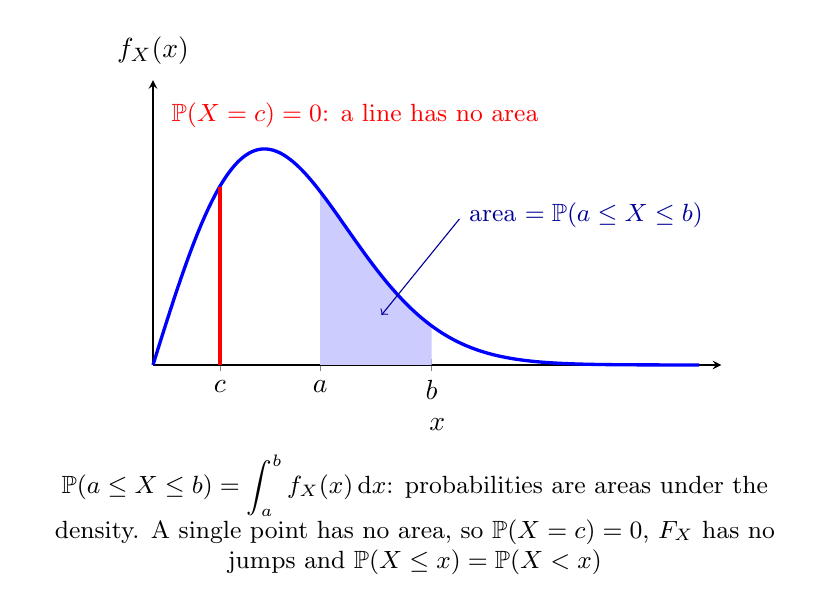
\begin{tikzpicture}
	\begin{axis}[
		axis lines=left, xmin=0, xmax=5.1, ymin=0, ymax=0.8,
		xtick={0.6,1.5,2.5}, xticklabels={$c$,$a$,$b$}, ytick=\empty,
		xlabel={$x$}, ylabel={$f_X(x)$}, ylabel style={rotate=-90, anchor=south, at={(axis description cs:0,1.02)}},
		samples=160, smooth, width=8.8cm, height=5.2cm, clip=false
		]
		\addplot[fill=blue!20, draw=none, domain=1.5:2.5] {x*exp(-x^2/2)} \closedcycle;
		\addplot[blue, very thick, domain=0:4.9] {x*exp(-x^2/2)};
		\draw[red, very thick] (axis cs:0.6,0) -- (axis cs:0.6,0.501);
		\node[red, font=\small, anchor=south west] at (axis cs:0.08,0.64) {$\mathbb{P}(X=c)=0$: a line has no area};
		\node[blue!60!black, font=\small, anchor=west] at (axis cs:2.75,0.42) {area $=\mathbb{P}(a\le X\le b)$};
		\draw[blue!60!black, ->] (axis cs:2.75,0.41) -- (axis cs:2.05,0.14);
	\end{axis}
	\node[anchor=north, font=\small, align=flush center, text width=9.6cm] at ([yshift=-2pt]current axis.outer south) {$\mathbb{P}(a\le X\le b)=\displaystyle\int_a^bf_X(x)\,\mathrm{d}x$: probabilities are areas under the density. A single point has no area, so $\mathbb{P}(X=c)=0$, $F_X$ has no jumps and $\mathbb{P}(X\le x)=\mathbb{P}(X<x)$};
\end{tikzpicture}
\end{document}
